% !TeX root = ../main.tex
% Add the above to each chapter to make compiling the PDF easier in some editors.

\chapter{Experiments and Results}\label{chapter:experiment}
In this chapter, we will describe the conducted experiment. The goal was to observe human reactions through image and audio recordings of the participants in conditions simulating exposure to different styles of humour delivered by a humanoid robot Roboy 3.0.

\section{Funboy Experiment}

To perform the experiment, we needed to expose the participants to a spoken Natural Language Dialogue with Roboy. The Roboy remarks could contain either conventional Ravestate dialogue utterances or humorous statements derived from the DeepComedian’s GPT-2 TLH model. We did not use any pre-generated humorous expressions due to two reasons. Firstly, it would introduce a noticeable variance in delay between the input \( U_{t-1}^i\) and output \( U_t^i\) depending on whether the output was pre-generated or not. Secondly, if the response \( U_t^i\) was pre-generated, we would not be able to incorporate reactive responses into the dialogue flow. Therefore, the system produced all humorous responses at runtime via the DeepComedian submodule. 

\subsection{Joke Categories}\label{section:expjokecat}

For the experiment, we conditioned the model using the following types of humour:
\begin{itemize}
    \item Size types: <|short|> and <|medium|>. Due to the speech synthesis computational cost, we decided to limit the size of the generated text. Otherwise, when the system produced a wave file containing synthesised speech, the cumulative delay would exceed 5 seconds, which we considered as a critical cut-off for the verbal exchange.
    \item Content types:
    \begin{itemize}
        \item <|chicken|> - \( c_1\): all samples for which the frequency of token "chicken" is higher than other tokens
        \item <|momma|> - \( c_2\): all samples for which the frequency of tokens "yo, momma", "your, momma" or "yo, mama" is higher than other tokens
        \item <|trump|> - \( c_3\): all samples for which the frequency of token "trump" is higher than other tokens
        \item <|pet|> - \( c_4\): all samples for which the frequency of tokens "pet", "cat" or "dog" is higher than other tokens
        \item <|army|> - \( c_5\): all samples for which the frequency of tokens "army", "military" or "soldier" is higher than other tokens
        \item <|police|> - \( c_6\): all samples for which the frequency of tokens "police" or "cop" is higher than other tokens 
        \item <|religion|> - \( c_7\): all samples for which the frequency of tokens "religion", "christian", "muslim", "jesus", "god", "buddha" is higher than other tokens
        \item <|bar|> - \( c_8\): all samples for which the frequency of tokens "bar", "barman" or "bartender" is higher than other tokens
        \item <|clown|> - \( c_9\): all samples for which the frequency of tokens "clown" or "circus" is higher than other tokens
        \item <|german|> - \( c_10\): all samples for which the frequency of token "german" is higher than other tokens
        \item <|boss|> - \( c_11\): all samples for which the frequency of token "boss" is higher than other tokens
        \item <|doctor|> - \( c_12\): all samples for which the frequency of tokens "doctor" or "nurse" is higher than other tokens
        \item <|british|> - \( c_13\): all samples for which the frequency of tokens "english", "british" or "brexit" is higher than other tokens
        \item <|cookie|> - \( c_14\): all samples for which the frequency of tokens "cookie", "biscuit" or "shortbread" is higher than other tokens
        \item <|family|> - \( c_15\): all samples for which the frequency of tokens "mom", "mum", "mama", "mother", "brother", "sister", "father", "grandfather", "granny", "grandpa", "grandmother", "grandma", "parent" or "family" is higher than other tokens
        \item <|friend|> - \( c_16\): all samples for which the frequency of token "friend" is higher than other tokens
        \item <|dadjokes|> - \( c_17\): all samples that belong to the subset of jokes derived from "r/dadjokes" subreddit but do not belong to other classes
        \item <|other|>  - \( c_18\): the rest of the samples
    \end{itemize}
\end{itemize}

\subsection{System Configuration}

In the experiment, we used Roboy 3.0 as the joking humanoid robot.

Hardware configuration setup comprised the following equipment:
\begin{itemize}
    \item Workstation running all local software:
    \begin{itemize}
        \item CPU: Ryzen 3900X
        \item GPU: Nvidia RTX 2080Ti
        \item RAM: 32 GB
    \end{itemize}
    \item Logitech HD Pro Webcam C920 camera to record images for \acrshort{ver} and speech for \acrshort{ser}
    \item Standalone microphone to record speech for \acrshort{asr}
    \item Loudspeaker for sound output 
    \item Projector for Roboy face projection
\end{itemize}

Software setup comprised the following modules and packages:
\begin{itemize}
    \item Software modules and packages:
    \begin{itemize}
        \item GPT-2 TLH based on GPT-2-L and trained for 100 000 iterations using the defined joke categories (see Section \ref{section:expjokecat})
        \item Ravestate 0.7.0 for Dialogue System capability including:
        \begin{itemize}
            \item Ravestate Funboy as the \acrshort{darvah} framework implementation
            \item Ravestate Wildtalk (version from 24.09.2019) running ConvAI GPT model
        \end{itemize}
        \item Docker running the following containers:
        \begin{itemize}
            \item Funboyn4j with Neo4j instance for the DARVAH ontology
            \item Rosemo with EmoPy and \acrshort{ser}
        \end{itemize}
        \item Roboy face Android application to provide face projection and facial emotion animations
        \item Roboy Socnreo for speech synthesis
        \item roboy\_speech\_recognition (Google) for speech recognition
    \end{itemize}
\end{itemize}

\subsection{Experiment Setup}\label{subsection:expset}

We conducted the experiment as a one-to-one conversation between a participant and the robot. The researcher explained the goal and the flow of the interaction to the participant before the start. The researcher was always present in the vicinity and controlled the beginning and the end of each experiment. Although we did not wholly restrict access to the room, we isolated the part of the room where the experiment took place from other people. A table separated Roboy from the participant who sat in the chair across.

We recorded each participant from a frontal view by a camera and microphone placed on Roboy while they were communicating. This was necessary to capture natural visual and audial cues as an involuntary response to humorous input. Although we did not specifically inform the participants about the conversation structure or that it would contain any comedic elements, all of the participants had an idea about the humorous component of the experiment.
There was no time limit for conversations. Thus, each participant could choose when to finish the interaction themselves. We structured the flow in each conversation in the following way:
\begin{enumerate}
    \item The greeting – in this part, after the participant greeted Roboy, Roboy greeted the participant.
    \item The conventional dialogue – in this part, Roboy asked or answered simple questions.
    \item The humour-enabled dialogue – in this part, Roboy started to use Funboy's \( D\) state to decide whether to tell jokes or use conventional responses. The part came into effect after 90 seconds since the start.
    \item The farewell - in this part, the participant finished the conversation by saying farewells to Roboy.
\end{enumerate}
We prepared this conversation structure to pursue two objectives. The first one was to observe how emotions and behaviour of the participants change when the robot starts joking. Thus, we did not start the Funboy's DARVAH loop immediately after the whole system start-up but introduced an 80 seconds delay so that the participants had a chance to experience a pure conventional Ravestate dialogue. 
    
During each conversation, we collected the image and audio streams and processed them at near real-time via rosemo models to obtain the classification of emotions expressed by the participant.
    
We collected the visual and audial information, under the assumption that they may contain behavioural patterns indicating responses to a humorous input which may lead to understanding if people are more willing to engage in an interaction with Roboy, given the conditions of the experiment.
 
The system continuously acquired latest \(w=\)10 seconds of recognised emotions from the image stream. We chose this size of the window via testing the setup before the experiment. Given that we configured rosemo.image to use a frequency of 2 fps\footnote{frames per second}, the \( V\) state received 20 latest samples each time the validation process occurred. We calculated the positivity value based on these samples to validate the emotion data for attuning the affinity scores. 

Although we recorded the speech as well, we encountered a certain problem trying to use the obtained emotion samples. Unfortunately, due to the delays in response and processing tasks on Roboy's side and the necessity to record the whole user input to recognise the emotions, we could not use the speech emotions predictions for calculating the positivity value considering the time elapsed from the moment we collected the data until we obtained a speech emotion recognition result. Therefore, in this experiment we had to select VideoOnly strategy in EmotionStrategy class to set parameter \( \beta = 0\) for the \acrshort{ser}.

After the interactive part of the experiment, we asked each subject to answer a set of questions designed to gauge their involvement in the process. 

\subsection{User Study Questions}

The questionnaire consists of 6 parts. The first one is a set of four questions on how anthropomorphic Roboy seemed to the participants. Each question offered a modified Likert scale from -2 to 2 and asked to rate the participant's impression of the robot according to the following scales:
\begin{itemize}
    \item Q 1.1. From Fake: -2 to Natural: 2.
    \item Q 1.2. From Machine-like: -2 to Human-like: 2.
    \item Q 1.3. From Unconscious: -2 to Conscious: 2.
    \item Q 1.4. From Artificial: -2 to Life-like: 2.
\end{itemize}

The second part offered five questions on how likeable Roboy appeared. Each question provided a modified Likert scale from -2 to 2 and asked to rate the participant's impression of Roboy according to the following scales:
\begin{itemize}
    \item Q 2.1. From Dislike: -2 to Like: 2.
    \item Q 2.2. From Unfriendly: -2 to Friendly: 2.
    \item Q 2.3. From Unkind: -2 to Kind: 2.
    \item Q 2.4. From Unpleasant: -2 to Pleasant: 2.
    \item Q 2.5. From Awful: -2 to Nice: 2.
\end{itemize}

The following set of questions consisted of seven fully formulated statements about Roboy and asked the respondents to rate their agreement on the standard Likert scale from 1 to 5 ("strongly disagree" to "strongly agree"):
\begin{itemize}
    \item Q 3.1. I enjoyed the robot talking to me.
    \item Q 3.2. I find the robot fascinating.
    \item Q 3.3. Talking with the robot was easy.
    \item Q 3.4. I consider the robot a pleasant conversational partner.
    \item Q 3.5. I find the robot pleasant to interact with.
    \item Q 3.6. I feel the robot understands me.
    \item Q 3.7. I think the robot is funny.
\end{itemize}

Questions Q4 and Q5 offered the participants to write their feedback in the free form regarding what they liked and didn't like about Roboy.

The last question consisted of three parts Q6.1, Q6.2 and Q6.3, which asked to briefly describe the respondents' emotions in the beginning, the middle and the end of the conversation with Roboy. This is the most essential part of the questionnaire because it directly asks to self-evaluate the person's emotions which are a necessary component of the experiment.

\section{Results of the Main Experiment}

In this section, we will discuss the results obtained from the Main Experiment. There were 13 participants - all of them are students in STEM fields at the Technical University of Munich. Most of the respondents were familiar with the Roboy project. Further, this section covers the performance of Funboy as well as the observations about the experiment. Regarding the materials collected by Rosemo, we will concentrate on the image data. In the second subsection, we explore the self-reported assessment from the User Study questionnaire and scrutinise the reports.

\subsection{Funboy Results}

We evaluated the performance of the Funboy system using the hardware mentioned above setup:
\begin{itemize}
    \item Speech synthesis took on average around 1 second using 600 Mbps Internet connection with about 9 ms ping to Google servers.
    \item EmoPy can recognise emotions on a single sample extracted from a Full HD frame (1920 x 1080 pixels) in 200 milliseconds. This means that to stay within near real-time constraints, we should require the sampling frequency \( f \leq 5 Hz\). In the experiment, we set the frequency to 2 Hz to have enough leverage on speed.
    \item For the \acrshort{ser}, it takes around 800 milliseconds to recognise a wave sample of 20 seconds (the time scales linearly).
    \item Joke generation was the most resource taxing task. The <|short|> joke type takes 3 seconds on average to generate a sample while the <|medium|> type jokes were taking over 5 seconds. 
\end{itemize}

Based on the data we recorded during the experiment, we could calculate the amount of time people spent talking with Roboy until the farewells. The mean conversation duration is \( \mu = 853\) seconds (while the standard deviation is \( \sigma = 431\)). Even the shortest conversation of 347 seconds was well over the delay value of the DARVAH loop start-up, which was 80 seconds. Therefore, we consider the conversation engagement to be satisfactory because most of the participants spent enough time to familiarise themselves with Funboy.

However, longer engagement time does not necessarily mean that the participants found conversing with Roboy rewarding. Although all of the participants were enthusiastic at the start of the conversation, only four of them were satisfied by the end of the experiment. 

9 out of 13 participants experienced troubles with the delay of the joke generation task between the input and output of the Ravestate Dialogue System - some of the respondents became too impatient and would repeat their remark several times.

All participants visually responded better to jokes that closely resembled canned comedy such as:
\begin{itemize}
    \item Why did the chicken cross the road?
    \item How many \( X\) does it take to screw in a light bulb?
    \item Yo momma is so \( X\), that she \( Y\)
\end{itemize}
Completely original jokes seemed to cause more confusion due to either being too noisy or puzzling to be perceived well.

Several participants asked the robot to repeat the previous joke or general statement during the conversation, which currently is impossible. This functionality might be useful even outside of the Funboy's DARVAH loop and should be implemented system-wide in Ravestate.

Overall, all participants wished for Roboy to be more expressive regarding the humour delivery to better distinguish between conventional conversation and humorous responses:
\begin{itemize}
    \item Use more facial expressions
    \item Use verbal confirmations in the humorous responses, such as starting the response with, for example:
    \begin{itemize}
        \item "I know a joke..."
        \item "Let me tell you a joke..."
        \item "Here is a joke..."
    \end{itemize}
    \item Introduce head movements into the delivery process
\end{itemize}

However, when asked whether they would prefer canned laughter over the current laugh token approach, most of the participant agreed that the current way of adding laughter to the response seems better.

Furthermore, it is interesting to compare two of the most different results concerning the calculated affinity scores in Table~\ref{table:er1} (see scores for all participants in Appendix~\ref{appendix:finalscores}).

User 0304J142142B spent 17 minutes 48 seconds, and User 0304L200631S spent 31 minutes 13 seconds talking to Roboy.
The first user heard 33 jokes, of which the only reaction to 7 was evaluated positively. Thus, the success rate is 0,21. For the second user, the number of generated jokes was 70, and all of them induced positive evaluations, which gives us the success rate of 1. These results demonstrate the difference in how individual respondents emotionally reacted to the generated humorous responses.

\begin{table}[htpb]
\centering
\begin{tabular}{|l|l|l|l|l|l|l|l|l|l|l|l|l|l|l|l|l|l|l|}
\hline
\multicolumn{19}{|c|}{Final Affinity Scores}                                         \\ \hline
User & \multicolumn{18}{c|}{Scores \{\(c_1\):\(c_{18}\)\}}                           \\ \hline
0304J142142B & 1 & 0 & 0 & 0 & 0 & 0 & 0 & 0 & 0 & 0 & 0 & 0 & 0 & 0 & 0 & 4 & 1 & 1 \\ \hline
0304L200631S & 0 & 2 & 1 & 4 & 4 & 4 & 5 & 5 & 4 & 6 & 4 & 4 & 7 & 5 & 2 & 1 & 3 & 9 \\ \hline
\end{tabular}
\caption{Final affinity scores for two participants after the experiment.}
\label{table:er1}
\end{table}

Regarding the EmoPy results, unfortunately, we encountered a substantial problem with Automatic Emotion Recognition results. Over the course of the whole experiment, the recognition results were continuously biased towards "calm" emotion (see Appendix~\ref{appendix:emopy}). Although we initially ignored neutral emotions such as calm and focused on validation using only binary "negative versus positive" emotions combinations approach, we cannot accept the current \acrlong{fer} result as reliable due to the demonstrated bias. There has to be another solution to tackle this problem in the future to be able to continue the research further.

We tried to identify the cause for such behaviour and arrived at the following possible reasons after examining our saved image data samples:
\begin{itemize}
    \item EmoPy's FERModel might be sensitive to uneven lighting
    \item the FERModel's performance may substantially degrade when encountering shadows on faces  
    \item the FER+ dataset used to train FERModel contains exaggerated facial expression samples which may skew the recognition results (see Figure \ref{fig:fer})
\end{itemize}
These hypotheses need to be evaluated in future research.

We could not use the SER data evaluation in validation process due to the constraints above (see Subsection~\ref{subsection:expset}). However, we recorded the audio streams and tested the recognition result. Unfortunately, the SER model also demonstrated a bias towards "neutral" emotion, although, the prediction was less continuously biased. The results for the two samples are given in Table~\ref{table:serexp}.

We tried to examine the reasons for such behaviour and formulated the following hypotheses:
\begin{itemize}
    \item the SER model might be sensitive to background noise
    \item the model was trained on native speakers data which might distort the recognition for speakers who exhibit accents
\end{itemize}
These additional hypotheses also need to be evaluated in future research.

\begin{table}[htpb]
\centering
\begin{tabular}{|l|l|l|}
\hline
\multicolumn{3}{|c|}{SER Evaluation} \\ \hline
Emotion      & Disgust    & Happy    \\ \hline
Angry        & 14         & 0        \\ \hline
Disgust      & 42         & 0        \\ \hline
Fear         & 0          & 0        \\ \hline
Happy        & 0          & 0        \\ \hline
Neutral      & 14         & 100      \\ \hline
Sad          & 28         & 0        \\ \hline
Surprise     & 0          & 0        \\ \hline
\end{tabular}
\caption{Examples of correct and incorrect recognition results by the SER.}
\label{table:serexp}
\end{table}

\begin{figure}[htpb]
  \centering
  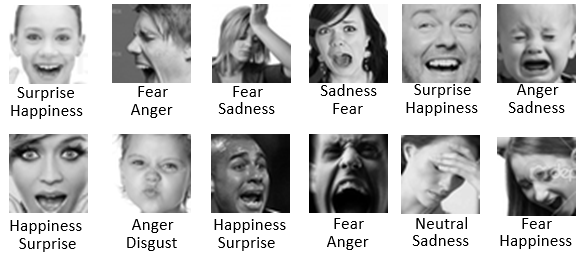
\includegraphics[width=0.8\textwidth]{figures/fer.png}
  \caption{Examples of images from FER/FER+ dataset \parencite{BarsoumICMI2016}.} \label{fig:fer}
\end{figure}


\subsection{User Study Results}

We gathered a succinct summary of the user feedback based on their answers to questions Q4 and Q5:
\begin{itemize}
    \item The participants liked the following features about Roboy: facial animations, voice, asking personal questions, some jokes were funny, understandable sentences, looks very cute, humour generation capability, diverse humour, entertaining conversation, mimics, dark humour.
    \item The participants didn't like these characteristics of Roboy: hard to distinguish between processing and listening, impossible to follow up on jokes, cannot repeat the previous response, sometimes the following response collides with the previous response, unfriendly, incoherent answers, delay in response, doesn't always understand the user's input, forgetful, interrupts the user, doesn't keep the context of the previous conversation.
\end{itemize}
Clearly, users had troubles with Roboy being incapable of following the conversation precisely. First of all, the Ravestate dialogue is missing the semantic context of the previously exchanged utterances in the conversation. Besides the contextual issues, the speech recognition service was not always properly recognising users' inputs, for example, interpreting "Hi, Roboy!" as "Jairo boy" or "Iowa". Additionally, the whole dialogue flow is still not good enough at being semantically precise regarding joke generation.

However, many participants also enjoyed that the robot tried to joke, although not always successfully. Also, the respondents reported that the facial animations were amusing. Several persons mentioned diverse humour and conversation flow as an advantage. Some of the users warned that several generated jokes might sound rude and offensive.

Furthermore, we calculated mean \( \mu\) and standard deviation \( \sigma\) values for the questions from part Q1 (see Table~\ref{table:us1}), Q2 (see Table~\ref{table:us2}) and Q3 (see Table~\ref{table:us3}). Observing these values, we derived the following conclusions. Firstly, the results of the first set of questions Q1.1 - Q1.4 almost negate each other regarding the evaluation of anthropomorphism by the participants. Every question's mean value is close to 0, which corresponds to being neutral on the modified Likert scale.

Concerning the next set of questions on likeability, we obtained slightly different results. First of all, the respondents were less in agreement about their scoring, given bigger standard deviation \( \sigma\) value. The mean values indicate a slightly positive leaning in the ratings with the values being between 0 and 1, which corresponds to being neutral and agreeing with statements on the modified Likert scale. The highest mean belongs to the question on "liking/disliking" Roboy. The lowest mean belongs to the question on Roboy's politeness.

The fully formulated statements about Roboy demonstrated more interesting results. Generally, the participants' ratings agreed the most on this part of the questionnaire with the standard deviation values between 0.96 and 1.08. The mean values for questions Q3.1 ("I enjoyed talking to the robot") and Q3.5 ("I find the robot pleasant to interact with") are 3.62 and 3.46 respectively which is in between "neutral" and "agree". Questions Q3.3 ("Talking with the robot was easy"), Q3.4 ("I consider the robot a pleasant conversational partner") and Q3.6 ("I feel the robot understands me") were rated below "neutral", therefore, most of the respondents leaned to disagree with the statements. However, people agreed on Roboy being fascinating and funny according to values \( \mu=4.08\) and \( \mu=4.00\) for questions Q3.2 ("I find the robot fascinating") and Q3.7 ("I think the robot is funny") respectively.

\begin{table}[htpb]
\centering
    \begin{tabular}{|l|l|l|}
    \hline
    \multicolumn{3}{|c|}{Anthropomorphism} \\ \hline
    Q  & Mean \( \mu\) & Std. Deviation \( \sigma\) \\ \hline
    1.1 & 0.08 & 1.04 \\ \hline
    1.2  & -0.08 & 1.32 \\ \hline
    1.3  & 0.15 & 0.99 \\ \hline
    1.4  & -0.38  & 1.04 \\ \hline
    \end{tabular}
\caption{Means and standard deviations of answers to the question on Anthropomorphism.}
\label{table:us1}
\end{table}

\begin{table}[htpb]
\centering
    \begin{tabular}{|l|l|l|}
    \hline
    \multicolumn{3}{|c|}{Likeability} \\ \hline
    Q   & Mean \( \mu\) & Std. Deviation \( \sigma\) \\ \hline
    2.1 & 0.85  & 1.14           \\ \hline
    2.2 & 0.38  & 1.45           \\ \hline
    2.3 & 0.31  & 1.25           \\ \hline
    2.4 & 0.23  & 1.36           \\ \hline
    2.5 & 0.54  & 1.13           \\ \hline
    \end{tabular}
\caption{Means and standard deviations of answers to the question on Likeability.}
\label{table:us2}
\end{table}

\begin{table}[htpb]
\centering
    \begin{tabular}{|l|l|l|}
    \hline
    \multicolumn{3}{|c|}{Acceptance} \\ \hline
    Q   & Mean \( \mu\) & Std. Deviation \( \sigma\) \\ \hline
    3.1 & 3.62  & 0.96           \\ \hline
    3.2 & 4.08  & 0.86           \\ \hline
    3.3 & 2.92  & 0.76           \\ \hline
    3.4 & 2.77  & 0.93           \\ \hline
    3.5 & 3.46  & 0.97           \\ \hline
    3.6 & 2.38  & 1.04           \\ \hline
    3.7 & 4.00  & 1.08           \\ \hline
    \end{tabular}
\caption{Means and standard deviations of answers to the question on Acceptance.}
\label{table:us3}
\end{table}

The last part of the questionnaire was devoted to emotion self-assessment. We compiled a summary of the reported answers in Table~\ref{table:us5}. Given the results, we arrived to the following conclusions:
\begin{itemize}
    \item Overall, 4 out of 13 participants reported feeling positive emotions over the whole experiment.
    \item 12 out of 13 participants felt positive at the beginning of the conversation and mostly split between being either curios or excited.  
    \item 7 participants who were excited about the experiment kept feeling positive by the middle of the conversation. 
    \item 5 out of 13 participant felt confusion in the middle of the conversation, which might have occurred due to assertive DARVAH behaviour.
    \item Most of the participants tried to make sense of noisy non-jokes which was mentally taxing and resulted in 9 participants experiencing negative emotions by the end of the conversation.
\end{itemize}

\begin{table}[]
\centering
    \begin{tabular}{|l|l|l|l|}
    \hline
    \multicolumn{4}{|c|}{Summary of Emotions} \\ \hline
    User           & Q 6.1  & Q 6.2  & Q 6.3  \\ \hline
    0228L160431P   & curious, excited & excited, frustrated & disappointed \\ \hline
    0228Y165728S   & interested & confused & frustrated \\ \hline
    0303D134007S   & excited & confused, laughing & exhausted \\ \hline
    0303D161701L   & happy, curious & happy, confused & happy, surprised\\ \hline
    0303J155544M   & regular & amused & amused \\ \hline
    0303M151400P   & curious & chill, happy & a bit frustrated \\ \hline
    0303M170134N   & nice, curious & confused & a bit tired \\ \hline
    0303P142946H   & interested & confused, happy & disappointed \\ \hline
    0303P201302N   & excited & interested & bored \\ \hline
    0303V145445S   & curious, excited & a bit uncomfortable, excited & a bit annoyed\\ \hline
    0304J142142B   & excited, happy & impressed, interested & satisfied \\ \hline
    0304L200631S   & curious, excited & curious, fun & curious, fun \\ \hline
    0304M152010H   & curious, excited & frustrated, amused & frustrated \\ \hline
    \end{tabular}
\caption{Summary of the self-reported emotions.}
\label{table:us5}
\end{table}

Based on the User Study self-assessment, we can consider the experiment to be moderately successful. However, we discovered many drawbacks that need to be fixed before conducting further research. Mainly, the DARVAH's decision state implementation in Funboy needs to be less aggressive regarding the positive decision-making, and the processing delays need to be lower.